\section{Slučajevi upotrebe}
\label{subsec:podnaslov2}
\subsection {Podnošenje zahteva za prijavu}
Proces registracije korisnika u auto školi započinje popunjavanjem online formulara, gde kandidat unosi svoje lične podatke. Administrativni radnik treba da proveri da kadnidat ispunjava potrebne uslove za upis i formira neophodnu dokumentaciju za kandidata. Nakon toga informacije prosleđuje administratoru sistema, koji unosi novog korisnika u bazu i prosleđuje radniku ID za trenutnog korisnika. Kada je kandidat prijavljen u auto školu, dobija imejl sa potvrdom o registraciji i svoj ID, pa se može ulogovati na svoj nalog. 

\subsubsection{Podnošenje prijave}
\label{subsubsec:prijava}
\begin{itemize}
  \item \textbf{Kratak opis}: Da bi kandidat započeo obuku u auto školi, prvo mora da podnese prijavu za upis. Popunjava online formular, gde unosi svoje lične podatke, koji se nakon potvrde šalju administrativnom radniku. Radnik formira dokumentaciju za kandidata i prosleđuje ih administratoru sistema, koji unosi informacije o kandidatu u sistem.
  \item \textbf{Učesnici}: 
    \begin{itemize} 
      \item Kandidat
      \item Administrativni radnik
      \item Administrator sistema
    \end{itemize} 
  \item \textbf{Preduslovi}:
    \begin{itemize}
    \item Kandidat mora posedovati važeću ličnu kartu.
    \item Kandidat mora uplatiti prvu ratu.
    \end{itemize}
  \item \textbf{Postuslovi}:
      \begin{itemize}
      \item Kandidat ispunjava uslove za prijavu.
      \end{itemize}
  \item \textbf{Osnovni tok}:
      \begin{enumerate}
        \item Kandidat otvara online formu za prijavu u auto školu.
        \item Sistem prikazuje formu kandidatu.
        \item Kandidat popunjava formu, unoseći sve potrebne informacije.
        \item Kanidat šalje unete podatke klikom na dugme “Pošalji”.
        \item Sistem validira unos podataka.
        \item Sistem čuva podatke.
        \item Sistem prosleđuje podatke administrativnom radniku.
        \item Аdministrativni radnik proverava da li kanidat ispunjava uslove za upis.
        \item Administrativni radnik formira dokumentaciju za kandidata.
        \item Administrativni radnik prosleđuje podatke o kandidatu administratoru sistema.
      \end{enumerate}

  \item \textbf{Alternativni tokovi}:
      \begin{itemize}
        \item A1. \textbf{Kandidat ne ispunjava uslove za upis.}
        Ukoliko je u koraku 4 administrativni radnik uočio da kandidat ne ispunjava uslove za prijavu i kontaktira ga kako bi ga obavestio o tome i ispravio podatke ukoliko je moguće. Proces se nastavlja u 1. koraku osnovnog toka.
      \end{itemize}

  \item \textbf{Dodatne informacije}:\newline
  Potrebni podaci za prijavu su ime, prezime, JMBG, broj telefona, imejl adresa i potvrda o uplati prve rate.
\end{itemize}

\begin{figure}[H]
  \begin{center}
      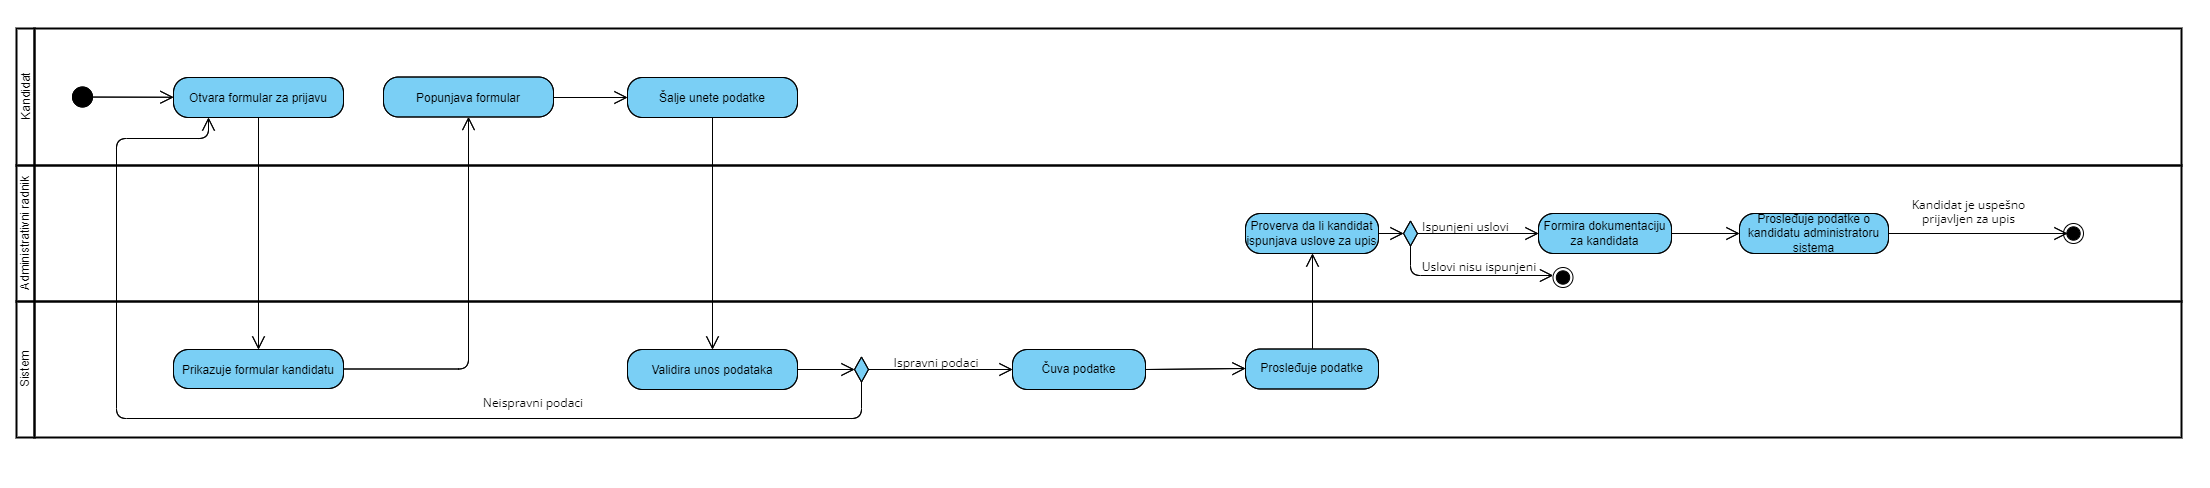
\includegraphics[width=140mm, height=70mm]{Diagrams/dijagram_aktivnosti_podnosenje_prijave.png}
  \end{center}
  \caption {Dijagram aktivnosti - Podnošenje prijave}
  \label{activity_podnosenje_prijave}

\end{figure}





\subsubsection{Registracija kandidata}
\label{subsubsec:registracija}
\begin{itemize}
  \item \textbf{Kratak opis}: Da bi kandidat mogao da se uloguje na svoj nalog i vidi svoje podatke, nepohodno je da dobije potvrdu da je upisan u auto školu, kao i nepohodan ID za logovanje.
  \item \textbf{Učesnici}:
  \begin{itemize}
    \item Kandidat
    \item Administrator sistema
    \item Administrativni radnik.
  \item \textbf{Preduslovi}:
    \begin{itemize}
    \item  Kandidat je popunio online prijavu.
    \item  Kandidat ispunjava uslove za upis.
    \end{itemize}
  \item \textbf{Postuslovi}:
      \begin{itemize}
      \item Kandidat je evidentiran u sistemu.
      \item Kandidat može da se prijavi na sistem.
      \end{itemize}
  \item \textbf{Osnovni tok}:
      \begin{enumerate}
        \item Administrator sistema prima informacije o novom kadnidatu.
        \item Administrator sistema unosi novog korisnika u bazu podataka.
        \item Sistem čuva unete podatke.
        \item Sistem šalje mejl novom kandidatu sa njegovim ID-jem.
        \item Sistem šalje mejl administrativnom radniku da je uspešno dodao novog kanidata.
        \item Administrativni radnik poziva kadnidata telefonom i proverava da li je dobio mejl sa svim potrebnim informacijama za prijavljivanje.
        \item Administrativni radnik ažurira spisak prijavljenih kandidata dodavanjem novog kadnidata.    
      \end{enumerate}

  \item \textbf{Alternativni tokovi}:
      \begin{itemize}
        \item A1. \textbf{Kandidat nije dobio mejl sa ID-jem i šifrom za pristupanje svom nalogu.}
        Ukoliko u koraku 4 kandidat nije dobio mejl, administrator sistema zahteva od sistema da ponovo pošalje mejl. Proces se nastavlja u koraku 4. osnovnog toka.
        \item A2. \textbf{Administrativni radnik ne može da kontaktira kadnidata.}
        Ukoliko u koraku 6 administrativni radnik ne može da stupi u kontakt sa kandidatom, trenutno stanje sistema se pamti i prekida se slučaj upotrebe na neko vreme. Naredni dan se slučaj upotrebe nastavlja ponovnim pozivom kandidata odnosno proces se nastavlja od 6. koraka osnovnog toka.
      \end{itemize}
\end{itemize}

\subsubsection{Raspoređivanje kandidata u grupu}
\label{subsubsec:grupe}
\begin{itemize}
  \item \textbf{Kratak opis}: Da bi kandidat bio raspoređen u grupu neophodno je da odabere neku od ponuđenih grupa, nakon logovanja na svoj nalog. 
  \item \textbf{Učesnici}: 
    \begin{itemize}
    \item  Kandidat - korisnik sistema koji bira grupu za teorijsku nastavu.
    \end{itemize}
  \item \textbf{Preduslovi}:
    \begin{itemize}
    \item Kandidat je dobio svoj ID i lozinku na mejl.
    \item Kandidat ima pristup internetu.
    \item Sistem je u funkciji.
    \end{itemize}
  \item \textbf{Postuslovi}:
      \begin{itemize}
      \item Kandidat je raspoređen u neku grupu.
      \end{itemize}
  
     
  \item \textbf{Osnovni tok}: 
      \begin{enumerate}
        \item Kandidat se prijavljuje na nalog.
        \item Kandidat klikom na dugme “Grupe” bira neku od ponuđenih grupa.
        \item Sistem šalje mejl kandidatu da je uspešno raspoređen u grupu i raspored održavanja časova.
        \item Kandidat dobija mejl sa podacima o grupi i rasporedu nastave.
      \end{enumerate}

  \item \textbf{Alternativni tokovi}:
      \begin{itemize}
        \item A1. \textbf{Neuspešno prijavljivanje.}
        Kandidat je pogrešio ID ili šifru u koraku 1, pa je nepohodno da proveri ispravnost podataka i da ih ponovo unese. Proces se nastvalja od koraka 1. osnovnog toka.
        \item A2. \textbf{Kandidat nije dobio mejl o raspoređivanju po grupama.}
        Kandidat nije raspoređen u željenu grupu, jer nije dobio mejl sa potvrdom u koraku 4, možda jer je vreme za prijavu isteklo (neko drugi je odabrao preostalo mesto). Proces se nastavlja od koraka 1. osnovnog toka.
      \end{itemize}


  \item \textbf{Specijalni zahtevi}:\newline
      Podaci koji su potrebni kako bi kandidat mogao da se uloguje su ID i lozinka u bazi.
\end{itemize}

  

\begin{figure}[H]
  \begin{center}
      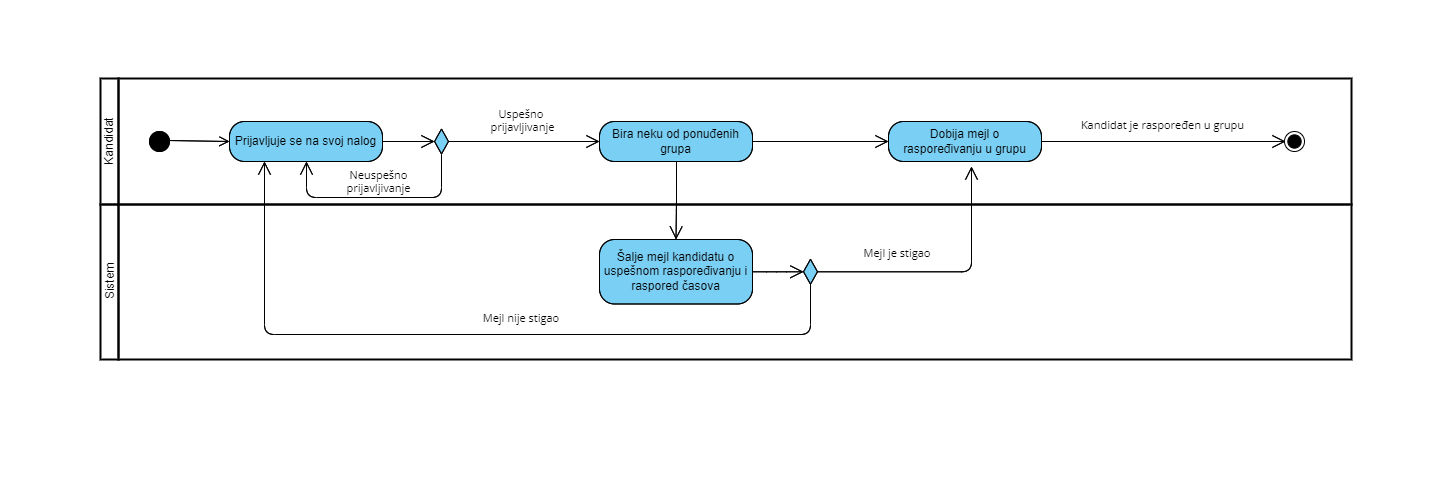
\includegraphics[width=140mm, height=70mm]{Diagrams/dijagram_aktivnosti_grupe.png}
  \end{center}
  \caption {Dijagram aktivnosti - Raspoređivanje kandidata u grupu}
  \label{activity_grupe}

\end{figure}


\subsection {Teorijska nastava}
Proces prijave za teorijsku nastavu kandidata, kao i vodjenje evidencije casova se odvija u okviru teorijske nastave. Takdoje, tu imamo i evidenciju polaganja kandidata koji su uspesno prijavili svoj ispit i odslusali casove predavanja.
s
\subsubsection{Teorijska nastava}
\label{subsubsec:prijava za nastavu}
\begin{itemize}
  \item \textbf{Kratak opis}: Kandidat koji se upisao u auto skolu pocinje sa pohadjanjem teorijske nastave u izabranoj grupi. Predavac evidentira prisustvo kandidata na casovima teorije koje on drzi.
  \item \textbf{Učesnici}:
    \begin{itemize}
    \item  Kandidat - korisnik sistema koji pohadja nastavu.
    \item  Predavac - korisnik koji drzi casove i evidentira prisustvo.
    \end{itemize}
  \item \textbf{Preduslovi}:
    \begin{itemize}
    \item  kandidat mora biti upisan u auto skolu.
    \item  kandidat mora biti rasporedjen u grupu kod predavaca.
    \item  kandidat je izmirio  prethodne troskove upisa.
    \item  predavac je zaduzen za grupu koju kandidati pohadjaju.
    \item  predavac je ulogovan na sistem.
    \item  sistem je dosutpan.
    \item  u sistemu ne postoji evidentiran cas za grupu u tekucem danu.
    \item  predavac  ima pristup internetu.
    \end{itemize}
  \item \textbf{Postuslovi}:
      \begin{itemize}
      \item Kandidat je evidentiran da je pohadjao nastavu.
      \item Predavac je evidnetirao odrzano predavanje.
      \end{itemize}
  \item \textbf{Osnovni tok}:
      \begin{enumerate}
        \item Predavac otvara stranicu za evidenciju prisustva korisnika.
        \item Predavac popunjava formular za zapocinjanje casa sa grupom.
        \item Predavac potvrdjuje da zapocinje cas sa grupom.
        \item Sistem prikazuje listu kandidata koji pohadjaju nastavu u toj grupi.
        \item Predavac evidentira prisustvo za svakog kandidata.
        \item Predavac zakljucuje evidenciju.
        \item Predavac zapocinje predavanje.
        \item Predavac nakon odrzanog cas zakljucuje cas.
        \item Sistem salje mail svim ucesnicima o uspeno zavrsenom casu i njihovom napretku.
      \end{enumerate}

  \item \textbf{Alternativni tokovi}:
      \begin{itemize}
        \item A1. \textbf{Neuspela validacija.}Ukoliku u koraku 2 sistem pronalazi neispravno polje formulara sistem obelezava polje koje treba ispraviti crvenom bojom, a ispod polja pise  uzrok neispravnosti. Nakon ponovnog ispravnog unosa podataka proces se nastavlja u koraku 3 osnovnog toka.s
      \end{itemize}
      
 \item \textbf{Dodatne informacije}:
      \begin{itemize}
        \item Polja formulara pri zapocinjanju cas su: Grupa, termin, cas.
      \end{itemize}
\end{itemize}

\subsubsection{Prijava za teorijski ispit}
\label{subsubsec:prijava za ispit}
\begin{itemize}
  \item \textbf{Kratak opis}: Kandidat nakon zavrsenog pohadjanja casova teorije podnosi prijavu za polaganje teorijskog ispita
  \item \textbf{Učesnici}:
    \begin{itemize}
    \item Kandidat korisnik sistema koji se prijavljuje za ispit
    \end{itemize}
  \item \textbf{Preduslovi}:
    \begin{itemize}
    \item  Kandidat mora biti upisan u auto skolu.
    \item  Kandidat je zavrsio-odslusao sve casove terojie.
    \item  Kandidat je izmirio prethodne troskove prijave.
    \item  Kandidat je ulogovan na sistem.
    \item  Sistem je dosutpan.
    \item  Kandidat ima pristup internetu.
    \end{itemize}
  \item \textbf{Postuslovi}:
      \begin{itemize}
      \item Kandidat je podneo prijavu za polaganje teorijskog ispita.
      \end{itemize}
  \item \textbf{Osnovni tok}:
      \begin{enumerate}
        \item Kandidat otvara stranicu za prijavu polaganja teorijskog ispita.
        \item Sistem prikazuje formular za prijavljivanje teorijskog ispita.
        \item Kandidata popunjava formular.
        \item Kandidat potvrdjuje prijavu klikom na dugme.
        \item Sistem evidnetira prijavu.
        \item Sistem salje mail kandidatu o uspesnoj prijavi.  
      \end{enumerate}

  \item \textbf{Alternativni tokovi}:
      \begin{itemize}
        \item A1. \textbf{Neuspela validacija.}
        Ukoliku u koraku 3 sistem pronalazi neispravno polje formulara sistem obelezava polje koje treba ispraviti crvenom bojom, a ispod polja pise  uzrok neispravnosti. Nakon ponovnog ispravnog unosa podataka proces se nastavlja u korakku 5.
      \end{itemize}
      
  \item \textbf{Dodatne informacije}:
      \begin{itemize}
        \item Polja formulara za prijavu: Ime, Prezime, JMBG, Datum poslednjeg casa, Predavac, Skenirana licna karata 
      \end{itemize}
\end{itemize}

\subsubsection{Izlazak na teorijski ispit}
\label{subsubsec:teorijski ispit}
\begin{itemize}
  \item \textbf{Kratak opis}: Kandidat koji je uspešno prijavio teorijski ispit izlazi na polaganje.
  \item \textbf{Učesnici}:
    \begin{itemize}
    \item Kandidat - korisnik sistema koji polaže ispit.
    \end{itemize}
  \item \textbf{Preduslovi}:
    \begin{itemize}
    \item  Kandidat mora biti upisan u auto školu.
    \item  Kandidat je odslušao sve časove teorije.
    \item  Kandidat je izmirio prethodne troškove prijave.
    \item  Kandidat je ulogovan na sistem.
    \item  Kandidat je uspešno prijavio teorijski ispit.
    \item  Sistem je u funkciji.
    \item  Kandidat ima pristup internetu.
    \end{itemize}
  \item \textbf{Postuslovi}:
      \begin{itemize}
      \item  Kandidat je je završio pohađanje teorijskog ispita.
      \end{itemize}
  \item \textbf{Osnovni tok}:
      \begin{enumerate}
        \item Kandidat je otvorio stranicu za polaganje teorijskog ispita.
        \item Sistem šalje na mail pristupnu lozinku za ispit.
        \item Kandidat unosi pristupnu lozinku.
        \item Sistem otvara stranicu sa teorijskim ispitom za kandidata.
        \item Kandidat potvrđuje da hoće da završi izradu ispita (ili je isteklo vreme za izvršavanje ispita).
        \item Sistem otvara stranicu sa rezultatima polaganja.
        \item Sistem šalje kandidatu mail sa ishodom polaganja za prijavu i rezultatima.
      \end{enumerate}

  \item \textbf{Alternativni tokovi}:
      \begin{itemize}
        \item A1. \textbf{Neuspela provera koda.}
        Neuspela provera koda: Ukoliko u koraku 3 kandidat unese loš pristupni kod polje za kod će postati crveno,
         i biće mu omogućeno da ponovo unese kod, ili da ponovno pošalje kod na mail. Kada ispravno unese kod proces se nastavlja u koraku 4.
      \end{itemize}
      
  \item \textbf{Specijalni zahtevi}:
      \begin{itemize}
        \item Polja formulara za prijavu: pristupni kod. 
      \end{itemize}
\end{itemize}

\begin{figure}[H]
  \begin{center}
      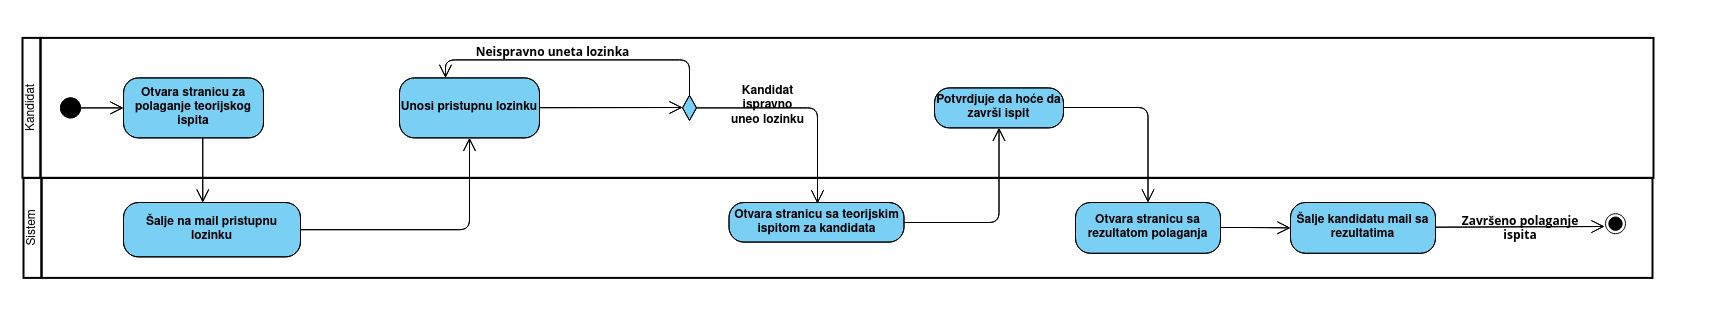
\includegraphics[width=140mm, height=70mm]{Diagrams/polaganje teorijskog ispita.png}
  \end{center}
  \caption {Dijagram aktivnosti - polaganje teorijskog ispita}
  \label{activity_polaganje_teorije}

\end{figure}


\subsection {Administracija}
Administrativni deo autoskole, vodjenje evidnecije o invenatru skole i ostalim pokretnostima i nepokretnostima.

\subsubsection{Evidencija voznog parak}
\label{subsubsec:vozni park}
\begin{itemize}
  \item \textbf{Kratak opis}: Organizator inventara ima mogucnost da vidi evidenciju svih kola i instruktora, i da vrsi promene u inventaru i rasporedu..
  \item \textbf{Učesnici}:
    \begin{itemize}
    \item Organizator inventara korisnik koji vrsi raspored inventara.
    \end{itemize}
  \item \textbf{Preduslovi}:
    \begin{itemize}
    \item  Organizator inventara je uspesno ulogovan na sistem auto skole..
    \item  Sistem je dosutpan.
    \item  Organizator inventara ima pristup internetu.
    \end{itemize}
  \item \textbf{Postuslovi}:
      \begin{itemize}
      \item  Organizator je azurirao vozni park i dodelio vozilima instruktores.
      \end{itemize}
  \item \textbf{Osnovni tok}:
      \begin{enumerate}
        \item  Organizator otvara stranicu za uvid voznog parka.
        \item Sistem prikazuje trenutni vozni park i informacije koji instruktro upravlja vozilom.
        \item Organizator je kliknuuo dugme izmeni na stranici.
        \item Sistem omogucava organizatoru da izmeni podatke u tabeli ili doda nove.
        \item Organizator potvrdjuje izmene.
        \item Sistem evidentira izmene.
        \item Sistem salje mail o izmenama instruktorima ako je doslo do novog rasporeda.
      \end{enumerate}

  \item \textbf{Alternativni tokovi}:
      \begin{itemize}
        \item A1. \textbf{Neuspela validacija.}
        Ukoliko u kkoraku 4 organizator u formu o izmenama unese nevalidne podatke polja formulara koja su neispravna ce biti crvena. Nakonsto organziator azurira podatke nastavlja se od koraka 5.
      \end{itemize}
      
  \item \textbf{Dodatne informacije}:
      \begin{itemize}
        \item Id auta, marka, reg broj, insturktor, kilometraza. 
      \end{itemize}
\end{itemize}